
\section{Schaltregler}

% % % % % % % % % % % % % % % % % % % %
% %Grundprinzip
% % % % % % % % % % % % % % % % % % % %
\subsection{Grundprinzip}
		Energie wird in verlustarmem Element zwischengespeichert und auf gewünschter
		Spannung stabilisiert. Als Energiespeicher kommen in Frage: \textbf{Kondensatoren}
		für kleine Leistungen und \textbf{Spulen} für mittlere bis grosse Leistungen.
		Übliche Schaltfrequenzen liegen im Bereich von $200kHz$. \\
		
		Energie wird im Magnetfeld gespeichert: $E_L = \dfrac{L}{2} \cdot i_L^2$ \\
		Spannung über Spule bewirkt Stromänderung: $i_L = \dfrac{1}{L} \int u_L(t) \, dt$ 
		oder $u_L = L \cdot \dfrac{d}{dt} i_L(t)$\\
		Kondensator am Ausgang stabilisiert Spannung ($E_C = \dfrac{1}{2} \cdot C \cdot U^2$)\\

% % % % % % % % % % % % % % % % % % % %
% %Arten von Wandler
% % % % % % % % % % % % % % % % % % % %
\subsection{Arten von Wandler}
		\begin{minipage}{8cm}
			\textbf{Abwärtswandler} (Step-Down, Buck Converter) \\
			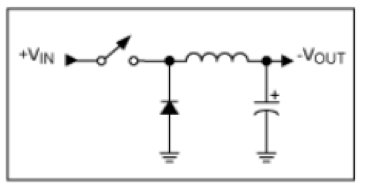
\includegraphics[width=6cm]{images/schaltregler/01_buckConv} \\
			\textbf{Invertierender Wandler} (Inverting) \\
			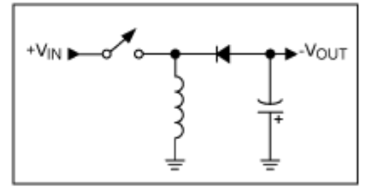
\includegraphics[width=6cm]{images/schaltregler/02_invConv} \\
		\end{minipage}
		\begin{minipage}{8cm}
			\textbf{Aufwärtswandler} (Step-Up, Boost Converter) \\
			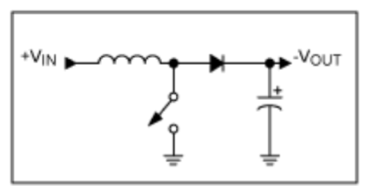
\includegraphics[width=6cm]{images/schaltregler/03_boostConv} \\
			\textbf{Sperrwandler} (Flyback Converter) \\
			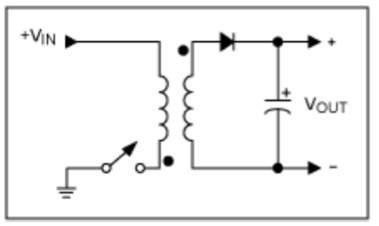
\includegraphics[width=6cm]{images/schaltregler/04_flybackConv}
		\end{minipage}

% % % % % % % % % % % % % % % % % % % %
% %Aufwärtswandler
% % % % % % % % % % % % % % % % % % % %
\subsection{Aufwärtswandler}
	\begin{minipage}{6cm}
		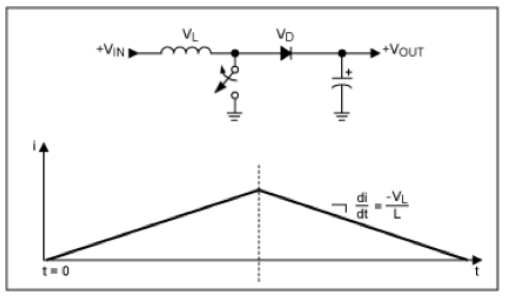
\includegraphics[width=6cm]{./images/schaltregler/05_boost-verhalten}
	\end{minipage}
	\begin{minipage}{12cm}
		\begin{tabular}{p{150pt} p{150pt} }
			Ladephase (Switch on)  & $\Delta I_{L_{on}}  = \frac{1}{L} \cdot U_{in} \cdot t_{on}$ \\
			Entladephase (Switch off) &$ \Delta I_{L_{off}} = \frac{1}{L} \cdot \left(U_{in}-U_{out}\right) \cdot t_{off} $\\
			Gleichgewicht &$ \Delta I_{L_{on}}  = -\Delta I_{L_{off}} $\\
			Ausgangsspannung	&$ U_{out}  = U_{in} \cdot \left( 1+\dfrac{t_{on}}{t_{off}}\right)$\\
		\end{tabular}
	\end{minipage}
	
% % % % % % % % % % % % % % % % % % % %
% %Abwärtswandler
% % % % % % % % % % % % % % % % % % % %
\subsection{Abwärtswandler}
	\begin{minipage}{4cm}
		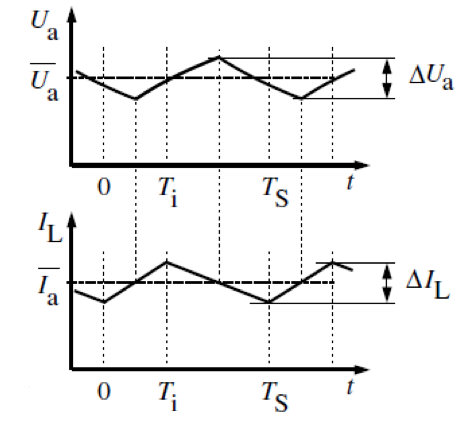
\includegraphics[width=4cm]{./images/schaltregler/06_buck-Verhalten}
	\end{minipage}
	\begin{minipage}{16cm}
		\begin{tabular}{p{100pt} p{250pt} }
			Schalter geschlossen & $\Delta I_{L_{on}} = \int_{0}^{T_i} (U_e - U_a) dt = \frac{1}{L} \cdot (U_e - U_a) \cdot T_i$ \\
			Schalter offen & $\Delta I_{L_{off}} = \int_{T_i}^{T_s}(U_a + U_{F_0}) dt = \frac{1}{L} \cdot (U_a - U_{F_0}) \cdot (T_s - T_i)$ \\
			Gleichgewicht & $\Delta I_{Lon} = \Delta I_{Loff}$\\
			Bilanz & $U_a = \frac{T_i}{T_s} \cdot U_e - \left(1-\frac{T_i}{T_s} \right) \cdot U_{F_0} \approx \frac{T_i}{T_s} \cdot U_e$\\
		\end{tabular}
	\end{minipage}
	
% % % % % % % % % % % % % % % % % % % %
% %Ladungsregler
% % % % % % % % % % % % % % % % % % % %	
\subsection{Ladungsregler}
% % % Phasenerklärung
\begin{tabular}{p{250pt}p{250pt}}
\hline
	\textbf{1. Phase}: S1,S2 geschlossen und S3,S4 offen.\newline
	über $C_1$: $Q_1 = C_1 \cdot U_{in}$\newline
	über $C_2$: $Q_2 = Q2$
	
	&
	\textbf{2. Phase}: S1,S2 offen und S3,S4 geschlossen.\newline
	über beiden $C$: $Q_{tot} = Q_1+Q_2$\newline
	über $C_2$: $Q_2 = \dfrac{C_2 \cdot Q_{tot}}{C_2+C_1}$\newline
	ergibt eine Spannung von $Uout = -\dfrac{Q_{tot}}{C_2+C_1 }$\\	
\hline
\end{tabular}	\\

	\begin{minipage}{250pt}
		Schaltbild:\\
		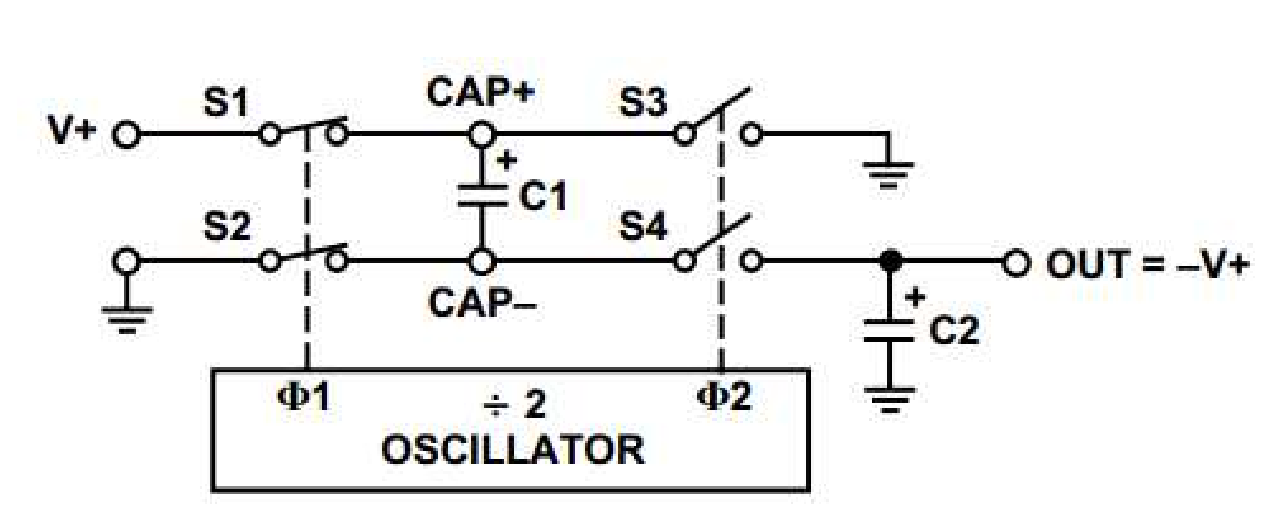
\includegraphics[width=6cm]{./images/schaltregler/07_chargepump}\\
		Ersatzschaltbild:\\
		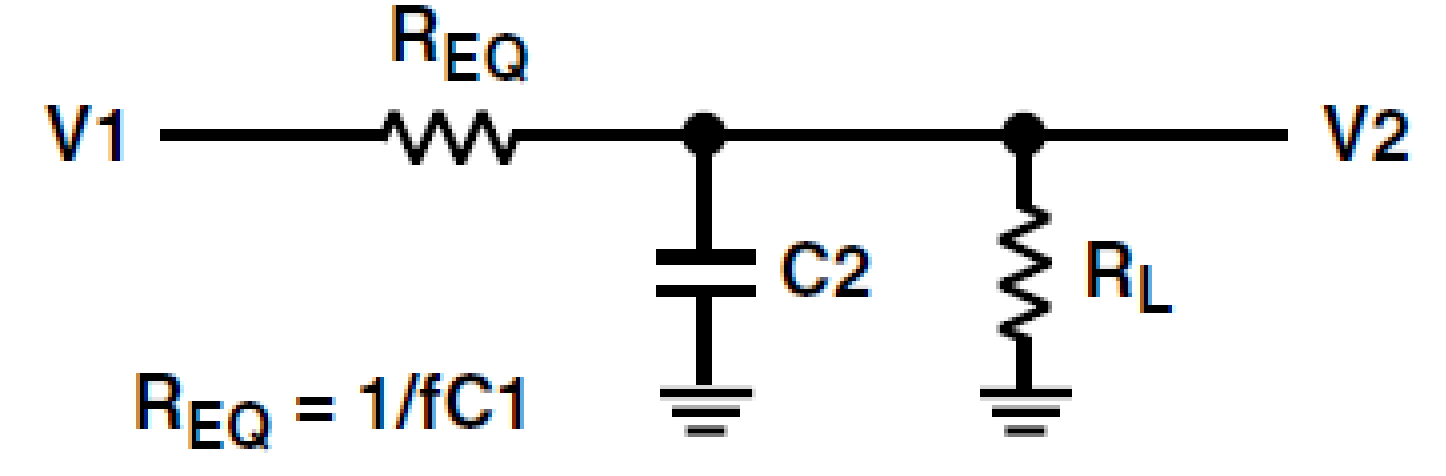
\includegraphics[width=6cm]{./images/schaltregler/08_lr_ersatzsb}
	\end{minipage}
	\begin{minipage}{250pt}
	Allgemeine Formeln:\\
			$\Delta U_a  = \frac{U_e - U_a}{1 + \frac{C_L}{C_1}} $\\
			$\Delta Q = C_L \cdot \Delta U_a = \frac{C_L \cdot C_1}{C_L + C_1} (U_e - U_a)$ \\
			$I_a = I_e = \frac{\Delta Q}{T_s} = \frac{C_L \cdot C_1}{C_L + C_1} \frac{U_e - U_a}{T_s}$\\\\
			
	Formeln fürs Ersatzschaltbild:\\
			Strom fliesst in "paketen": $dQ = C_1 \cdot dV$\\
			$I = \dfrac{V_1-V_2}{\frac{1}{f\cdot C_1}} = \dfrac{V_1-V_2}{R_{EQ}}$\\
			$R_{EQ} = \dfrac{1}{f\cdot C_1}$\\
			
	\end{minipage}\\
	

	